\chapter{System Overview}

\section{Vector graphics in hardware}

Based on initial research into vector graphics, the group decided to implement support for three types of primitives; lines, quadratic and qubic bezier curves.

\section{Architectual structure}

\begin{figure}[h!]
    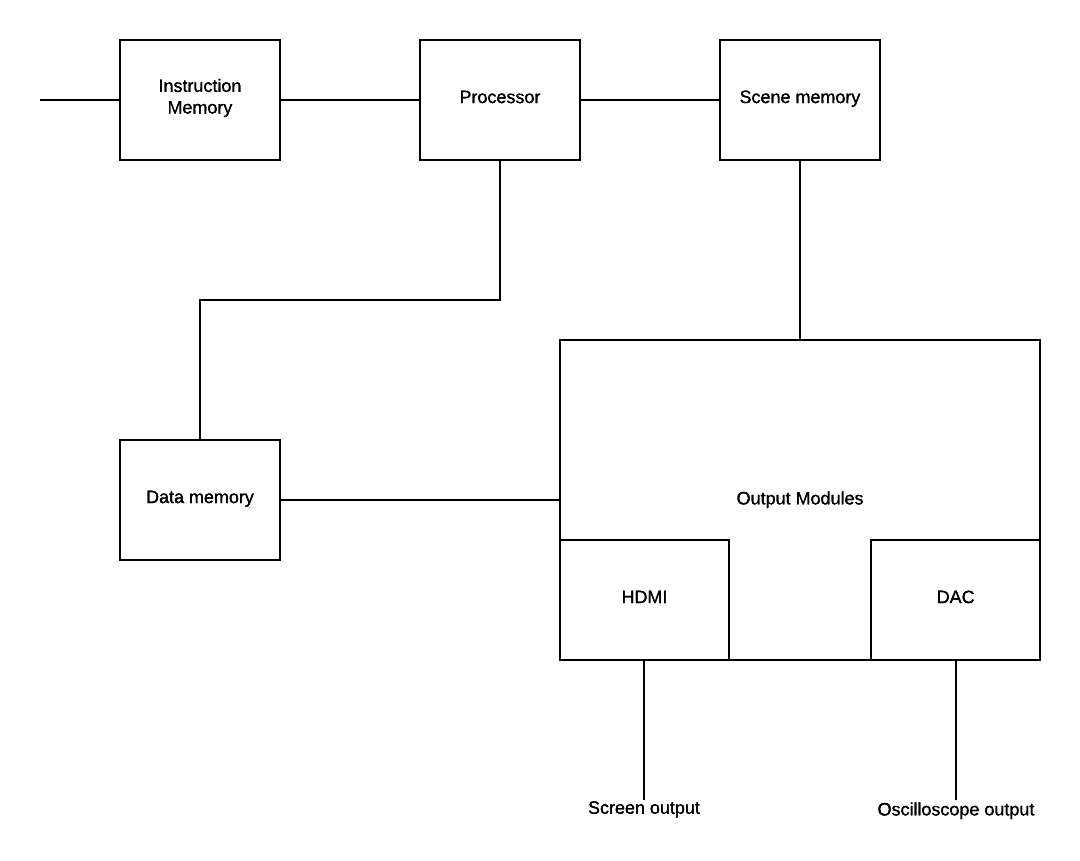
\includegraphics[width=\linewidth]{images/system-overview.png}
    \caption{A logical overview of the \vthreek architecture}
    \label{fig:system-overview}
\end{figure}

Figure \ref{fig:system-overview} shows how the major building blocks of the \vthreek architecture come together on a conceptual level.
Separation of instruction and data memory makes it a Harvard-like architecture.
The processor reads from instruction memory, executes instructions and adds/updates vector primitives in the scene memory.
Preprocessing these primitives for output is done by the output modules.

\section{Vector Graphics in Hardware}

This section gives an overview of how vector graphics is represented in the \vthreek architecture.
Later sections describe how the architecture processes and produces output based on this representation.

\subsection{Primitives}

The \vthreek architecture supports 3 basic primitives: lines, quadratic Bézier curves and cubic Bézier curves.
Lines are represented as linear Bézier curves.

\begin{figure}[h!]
    \centering
    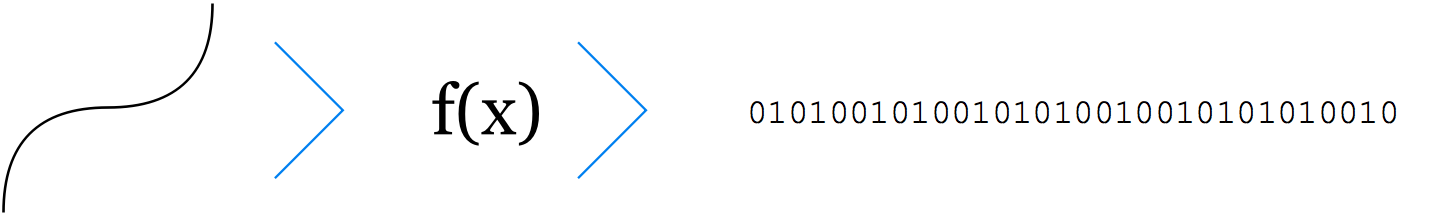
\includegraphics[width=0.85\linewidth]{images/primitive_encoding.png}
    \caption{Deciding upon an encoding scheme for vector primitives was one of the first decisions the group had to make.}
    \label{fig:primitive_encoding}
\end{figure}

Each primitives type is identified by the eight first bits.
To store a position on the screen, 32 bits is required: 16 bit for X and 16 bit for Y.
A line is represented by a start point and an end point.
To represent a quadratic Bézier curve a total of three points are needed, a start point, a control point and an end point.
The cubic Bézier curve includes one extra control point compared to the quadratic curve.
Table \ref{tbl:primitives} illustrates how each primitive is encoded as a binary string.

With the basic primitives linear, quadratic, and cubic Bézier curves, most other shapes can be constructed.
A square can be represented as four lines, a circle as multiple Bézier curves, and so on.

\begin{table}[h]
    \centering
    \begin{tabularx}{\linewidth}{|l|X|X|X|X|X|X|X|X|X|}
    \hline
    Primitive type (8) & x (16) & y (16) & x (16) & y (16) & x (16) & y (16) & x (16) & y (16) & Total bits \\ \hline
    Linear Bézier    & \(p_0^x \) & \(p_0^y \) & \(p_1^x \) & \(p_1^y \) & ~   & ~   & ~   & ~   & 72    \\ \hline
    Quadratic Bézier & \(p_0^x \) & \(p_0^y \) & \(p_1^x \) & \(p_1^y \) & \(p_2^x \) & \(p_2^y \) & ~   & ~   & 104   \\ \hline
    Cubic Bézier     & \(p_0^x \) & \(p_0^y \) & \(p_1^x \) & \(p_1^y \) & \(p_2^x \) & \(p_2^y \) & \(p_3^x \) & \(p_3^y \) & 136   \\ \hline
  \end{tabularx}
    \caption{Binary encoding of primitives. Bit size in parenthesis.}
	\label{tbl:primitives}
\end{table}

\subsection{Vector Images}

A vector image, or a scene, is a 2D canvas of fixed width and height on which primitives are placed.
The \vthreek architecture represents a scene conceptually as a collection of primitives.
Since primitives are represented with 16-bit integer coordinate-components, scene dimension is $65535 * 65535$.
This conceptual representation maps to a 1024 word deep, 136 bit wide, dual port scene memory module implemented using block RAM \cite{xilinx-block-ram} on the FPGA.
Since the size of the scene memory is static, the architecture maintains a primitive counter, indicating how many primitives are actually in the scene at any given time.


\section{Programming Model}

The \vthreek architecture is fairly conventional and largely RISC-inspired.
This makes its programming model similar to that of other modern computers.

A .v3k program is assembled on a host machine, transferred to the microcontroller which in turn loads it into instruction memory.
As previously mentioned, the \vthreek architecture is general, and as such, offers support for integer arithmetic, load/store instructions and simple branching.
Additionally, instructions for adding and processing vector primitives such as lines and curves are available.
A complete description of the \vthreek ISA is available in appendix \ref{app:isa}.

\subsection{A Simple \vthreek Program}

\begin{lstlisting}[label=lst:simple-program]
mov r1, #0
lsl r1, r1, #16
mov r1, #0

mov r2, #65535
lsl r2, #16
mov r2, #65535

line r1, r2
strp #0x00000001
\end{lstlisting}

Listing \ref{lst:simple-program} shows a very simple \vthreek program.
It simply draws a line across the scene, from bottom left corner to top right.

Vector primitives consist of a varying number of integer numbers.
In the case of a line, it consists of four 16-bit integers, \texttt{start\_x, start\_y, stop\_x, stop\_y}.
To utilize registers efficiently, each 32-bit register is loaded with one x,y coordinate-pair.

The first three lines put the coordinates $0,0$ in register \texttt{r1}, the next three puts $65535,65535$ in register \texttt{r2}.
The values in the registers are then used to create a line starting at \texttt{r1} and ending at \texttt{r2}.
Finally, the line is written to the scene memory using \texttt{strp}.
The output modules can now update their displays.

Upon creating a primitive with \texttt{line}, \texttt{bezquad} or \texttt{bezqube}, the resulting primitive is stored in a special purpose register in the processor.
To actually add the primitive to the scene, it has to be written to the scene memory using \texttt{strp}.
Primitives can also be loaded from the scene to be modified or processed using \texttt{ldrp}.
Only one primitive can be active in the processor at a time.

\subsection{More advanced programs}

// TODO: Write some actually more complex programs and document them.
